\title{Comp220 Proposal}
\author{
        Matthew Shaw\\
        ms228668\\
}
\date{\today}

\documentclass[12pt]{article}

\usepackage{tikz}
\usepackage{graphicx}

\begin{document}
\maketitle

\section{Outline of intended artifact}
\subsection{Area for improvement}
Too many games these days are focused around the boring 3d Euclidean space, simply because it's the one we happen to live in.
What I propose is a puzzle game, similar to Portal, where the player will navigate a 4 dimensional space, aiming to reach the end of each level, then proceed on to the next one.
This world would have an extra spatial dimension that the world we currently exist in. 
Doing so allows the puzzles to involve hiding things in different 4D spaces, which are impossible to see from the player's normal perspective.

\subsection{Approaches to the problem}
There are two main schools of thought for showing 4d hypershapes in 3d space: Projection and Slicing. 
\paragraph{Projection}
In the projection method, the entire shape is crushed down into 3d space, allowing all parts of it to be seen at once. 
This gives rise to the classic tesseract shape of a hypercube, which apears to be a small cube inside a larger cube. \\

\begin{figure}
    \centering
    \begin{tikzpicture}[scale=1.5]
        \draw (0,0) -- (3,0) -- (3,3) -- (0,3) -- cycle;
        \draw (1,1) -- (2,1) -- (2,2) -- (1,2) -- cycle;
        \draw (0,0) -- (1,1);
        \draw (3,0) -- (2,1);
        \draw (3,3) -- (2,2);
        \draw (0,3) -- (1,2);
    \end{tikzpicture}
    \caption{Shadow of a wireframe cube} \label{fig:CubeProjection}
\end{figure}

\begin{figure}
    \centering
    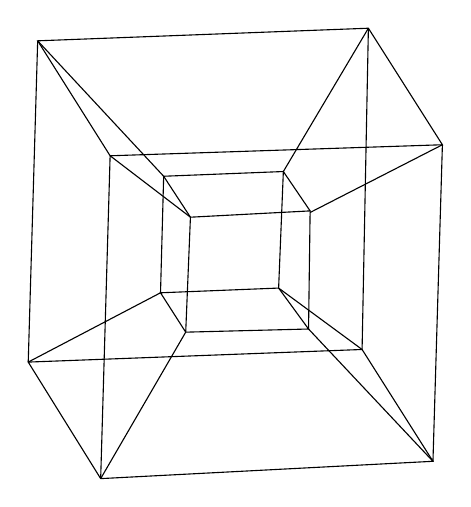
\begin{tikzpicture}[scale=2]
        %top and bottom squares
        \draw (0.55, 0.07) -- (2.66, 0.18) -- (2.21, 0.89) -- (0.09, 0.81) -- cycle; %abcd
        \draw (0.61, 2.12) -- (2.72, 2.19) -- (2.25, 2.93) -- (0.15, 2.85) -- cycle; %efhg
        \draw (1.09, 1.00) -- (1.87, 1.02) -- (1.68, 1.28) -- (0.93, 1.25) -- cycle; %ijlk
        \draw (1.12, 1.73) -- (1.88, 1.77) -- (1.71, 2.02) -- (0.95, 1.99) -- cycle; %mnpo
        %join top and bottom squares
        \draw (0.55, 0.07) -- (0.61, 2.12);
        \draw (2.66, 0.18) -- (2.72, 2.19);
        \draw (0.09, 0.81) -- (0.15, 2.85);
        \draw (2.21, 0.89) -- (2.25, 2.93);
        \draw (1.09, 1.00) -- (1.12, 1.73);
        \draw (1.87, 1.02) -- (1.88, 1.77);
        \draw (0.93, 1.25) -- (0.95, 1.99);
        \draw (1.68, 1.28) -- (1.71, 2.02);
        %inner to outer lines
        \draw (0.55, 0.07) -- (1.09, 1.00); %ai
        \draw (2.66, 0.18) -- (1.87, 1.02); %bj
        \draw (0.09, 0.81) -- (0.93, 1.25);
        \draw (2.21, 0.89) -- (1.68, 1.28);
        \draw (0.61, 2.12) -- (1.12, 1.73);
        \draw (2.72, 2.19) -- (1.88, 1.76);
        \draw (0.15, 2.85) -- (0.95, 1.99);
        \draw (2.25, 2.93) -- (1.71, 2.02);
    \end{tikzpicture}
    \caption{Shadow of a wireframe tesseract}\label{fig:TesseractProjection}
\end{figure}

In Figure~\ref{fig:TesseractProjection}, both the inner and outer cubes are the same size, one is just farther away along the 4th axis.
It is analogous to how in Figure~\ref{fig:CubeProjection}, one square is smaller than the other, even though they would be the same size in the real cube.\\
In addition to this, all the pyramid-shaped areas in Figure~\ref{fig:TesseractProjection} are cubes, like how the trapezoids in Figure~\ref{fig:CubeProjection} are actually squares.

\paragraph{Slicing}
The other method is simply taking a 3d cross-section of the hypershape. This is like cutting a 3d shape with a knife, and looking at the shape of the cut.
If a cube is cut in line with one of the sides, the cross section will be a square.
Similarly, if a tesseract is cut in line with one of it's faces, the cross-section will be a cube.
This would show a hypercube just as a normal cube, and would not allow the viewing of all parts of the hypershape at the same time, which is a lot easier for a person to see and understand, but an additional control is needed to move through the 4th dimension.

\subsection{Benefits of suggested approach}
When I do this, I would prefer the slicing method over projection. 
This view is more intuitive from a 3d perspective, as looking at it would be akin to looking at a 3d scene. 
However, moving along the 4th dimension would make the shapes appear to morph and shift, when in reality they are simply being moved.

\subsection{Potential challenges}
4D maths is very hard, and I have been working on and off on it for over a year now, without significant headway being made. 
However, since this is actually being done for the university now, I should be able to get more support from university staff with this matter, which should help me along massively.\\
The player might also have trouble understanding what is going on when they move through the 4th dimension. I could try to mitigate this through storytelling or tutorials, and through the visuals.
I could try fading the geometry along the 4th dimension, so that the player could see it fading in and out, however that may make it hard to discern what is passable and not.

\section{Broader context}
In my opinion, I feel like there aren't enough games set in the 4th dimension like this.
I believe that the largest one is Miegakure, however that has been in development since 2009, with no final release date in sight.\\
\begin{figure}
    \centering
    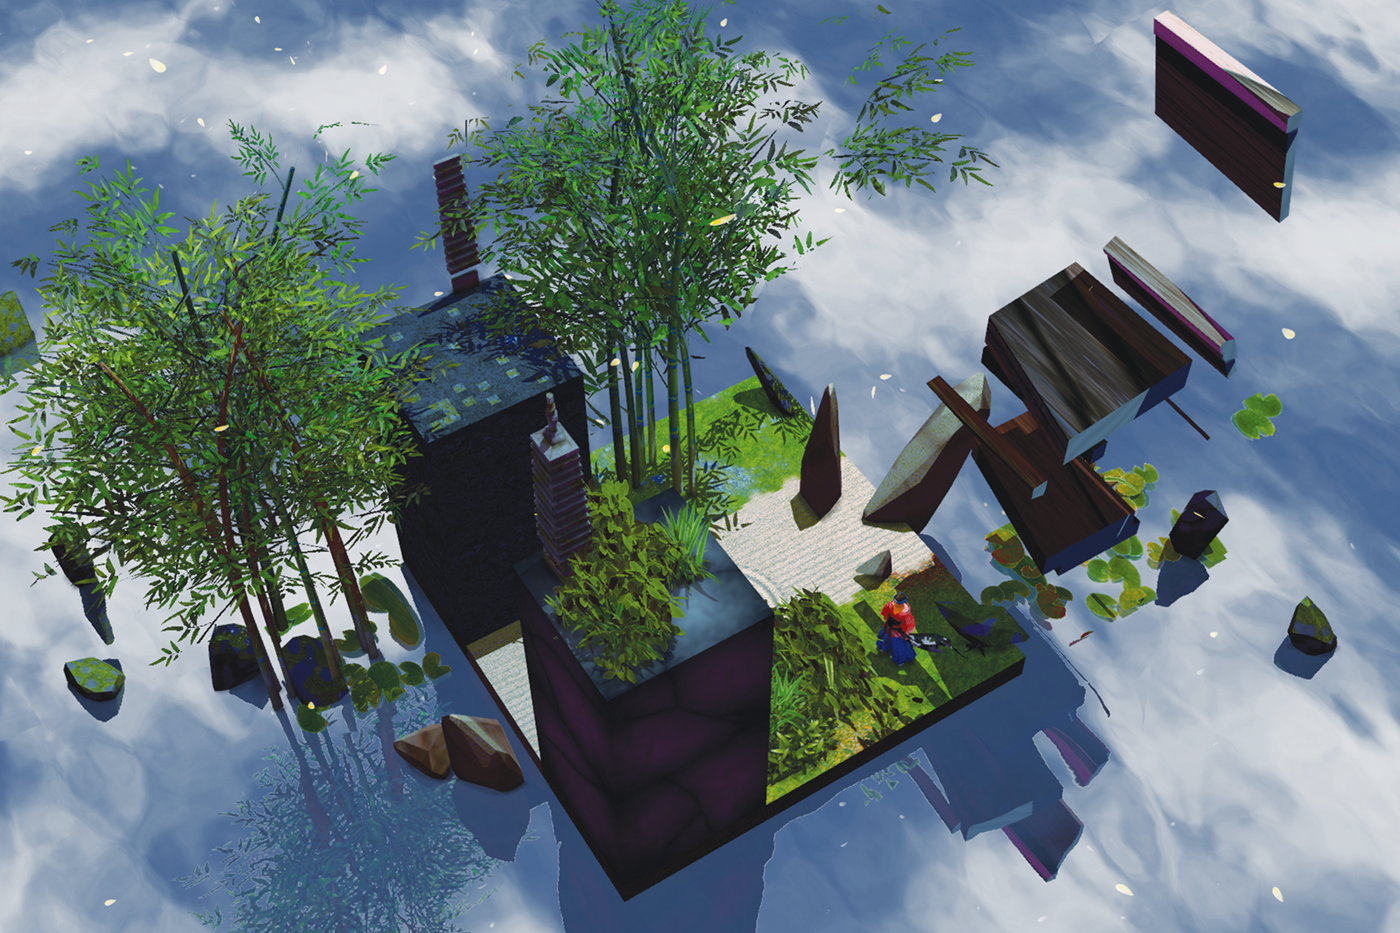
\includegraphics[width=\textwidth]{Media/Miegakure.png}
    \caption{Miegakure}
\end{figure}
There are also not a huge amount of games that defy normal space in general. The most popular are probably the Portal series, which link two normally separate spaces together via a portal.
There are also games like Manifold Garden or Antichamber, which mess with space and reality in their own way, but they aren't set in the 4th dimension.

\begin{figure}
    \centering
    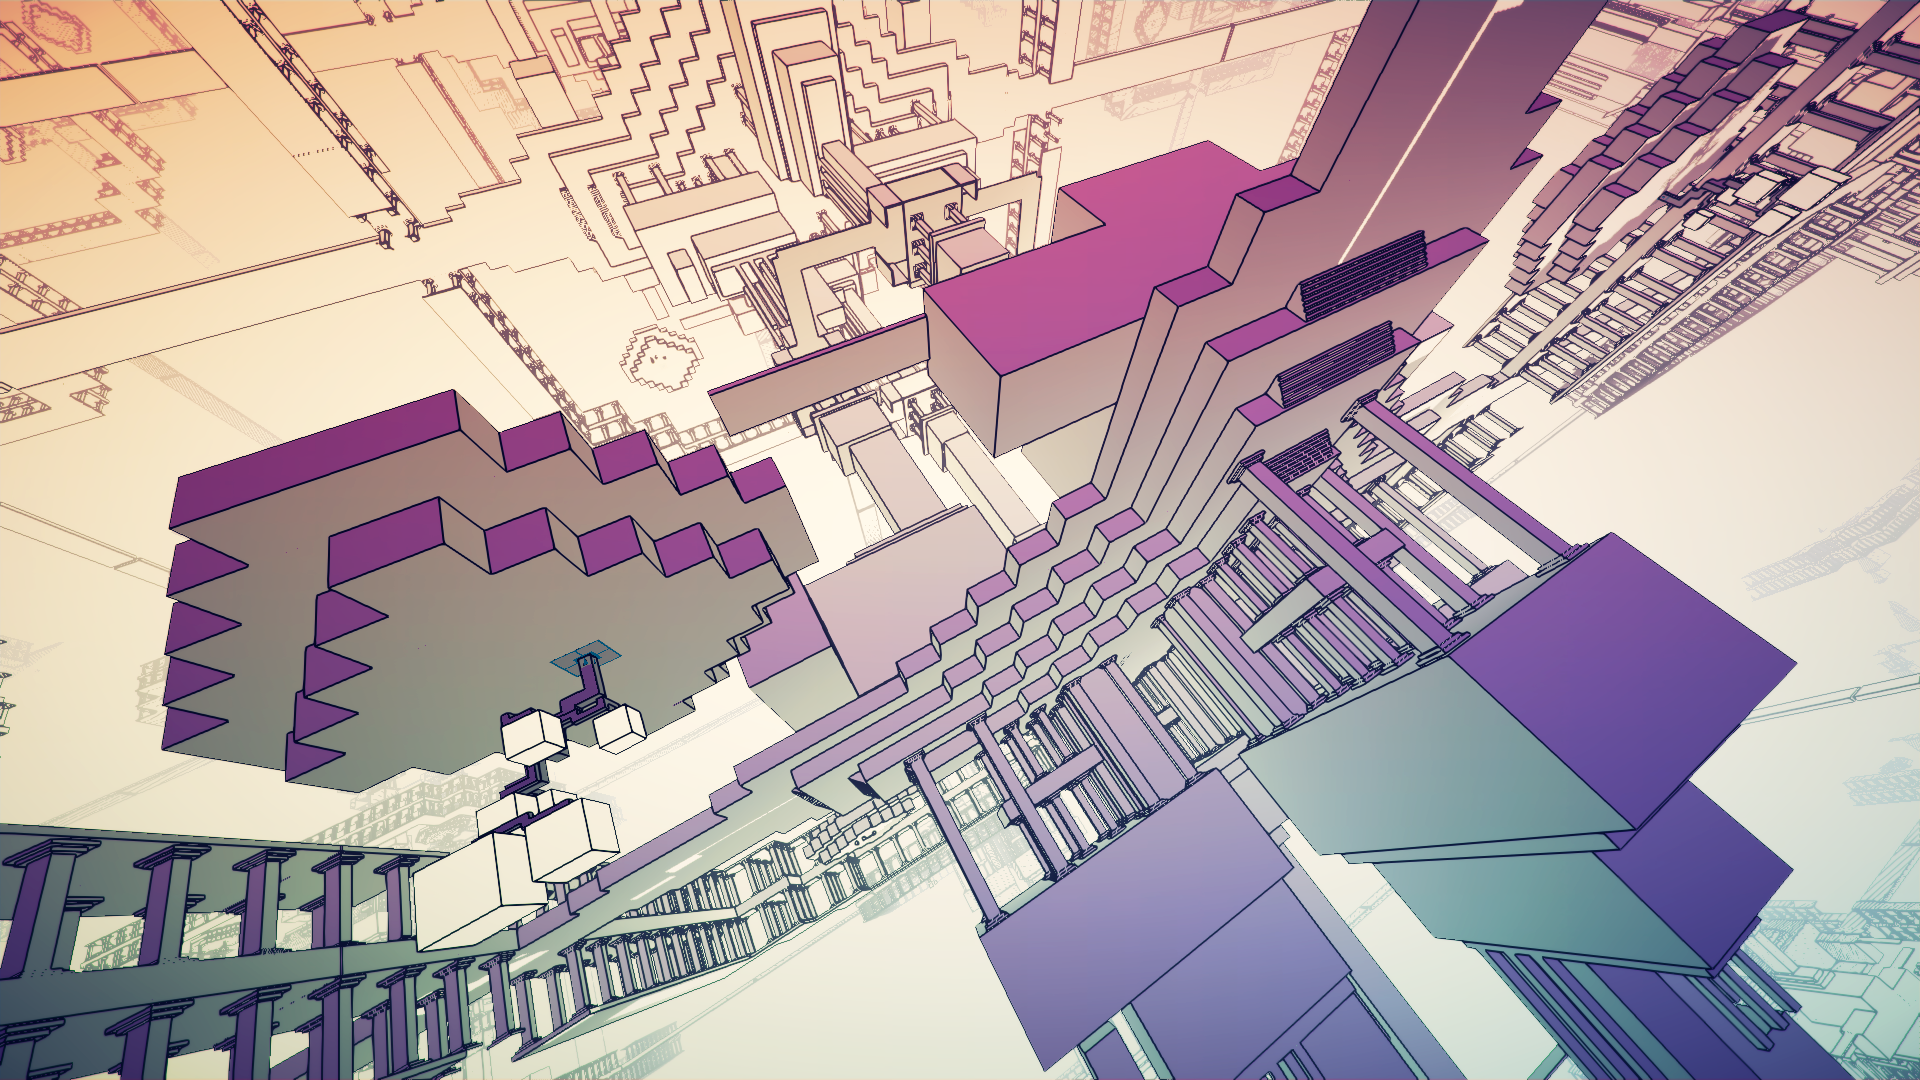
\includegraphics[width=\textwidth]{Media/ManifoldGarden.png}
    \caption{Manifold Garden}
\end{figure}
\begin{figure}
    \centering
    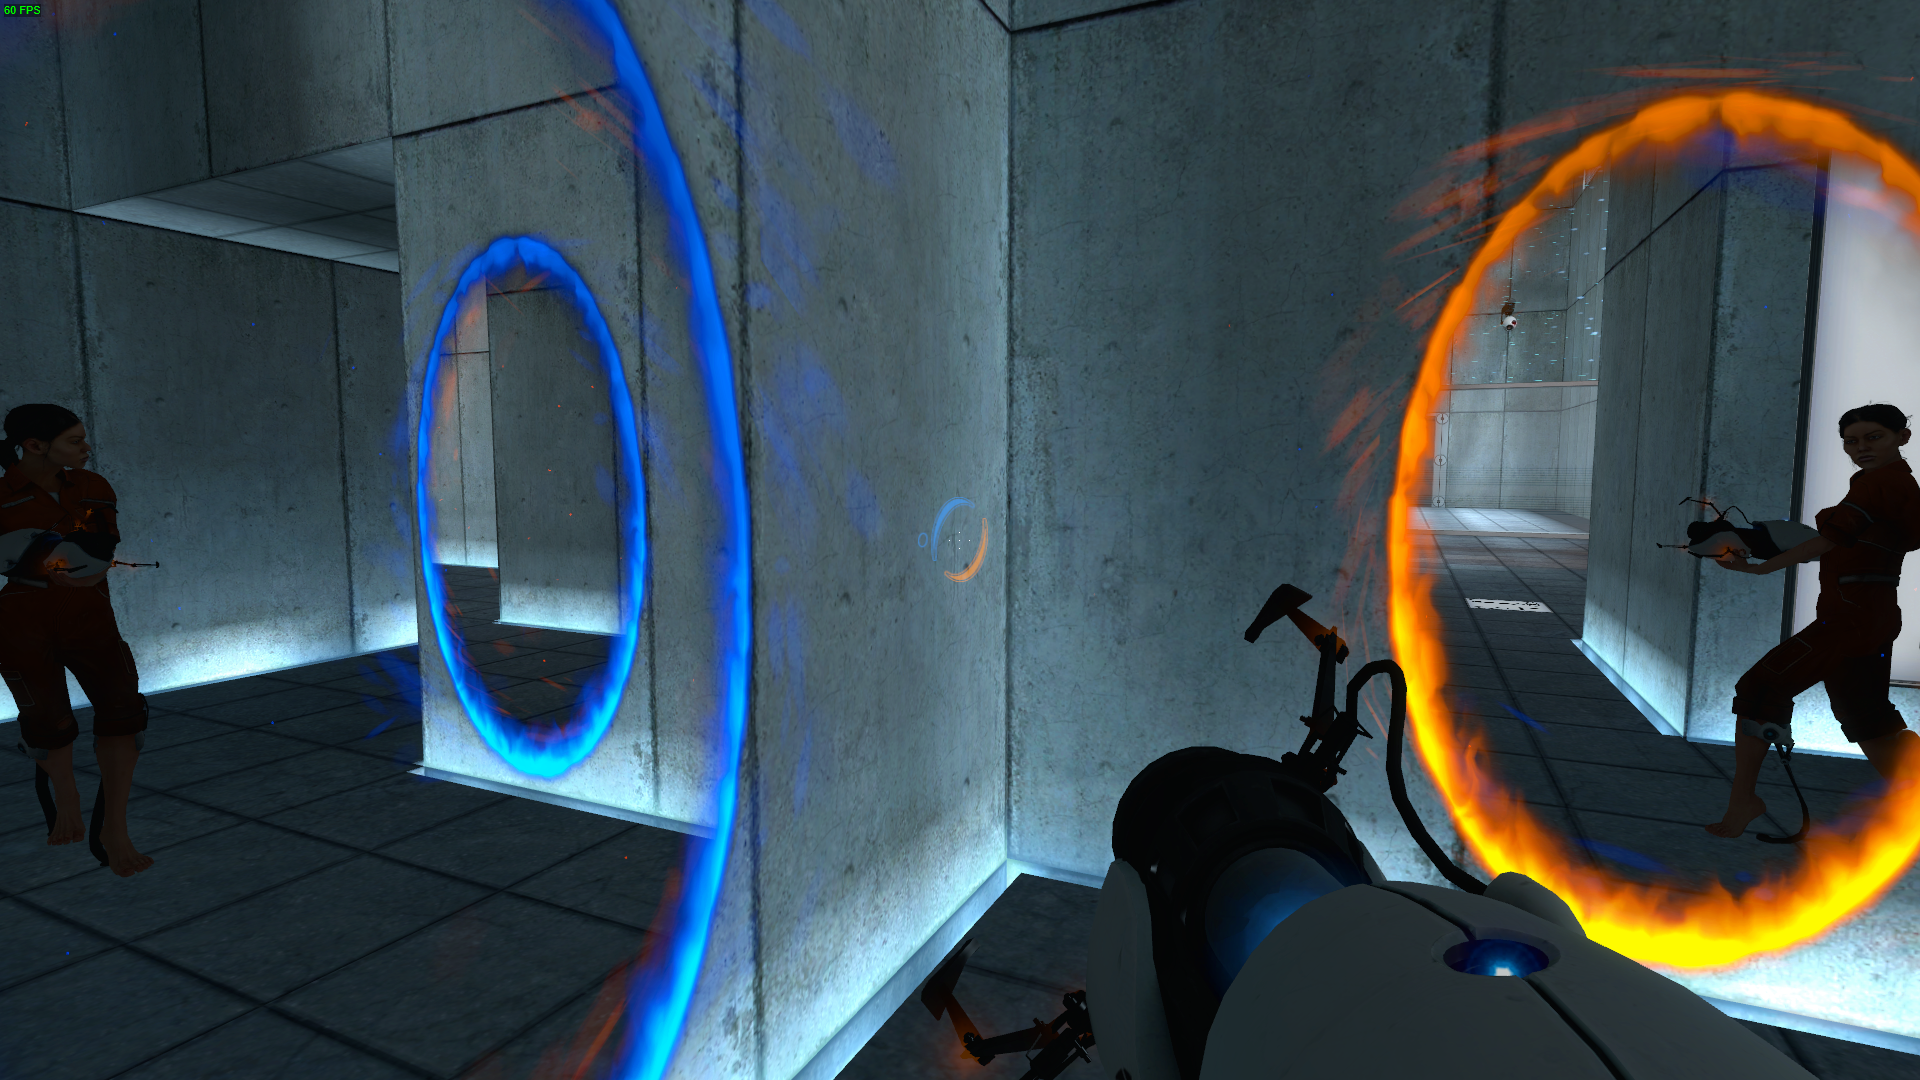
\includegraphics[width=\textwidth]{Media/Portal.png}
    \caption{Portal}
\end{figure}

Part of what I want to do with games is create novel experiences, and while 4D is not an completely new concept in games, its still relatively unexplored.
Maybe after creating it, ill find there is a very good reason why nobody wants games like this, but I can;t really know until I try it.

\section{Project feasability}
I believe that this is a project that it is possible for me to complete. While in the past I have struggled with this kind of maths, I am confident that I have improved in my abilities.

\subsection{Breakdown}
The hardest part of this will be to compute the 3d intersection of the 4d shapes.
However, as long as the cutting plane is not rotated, and remains orthogonal to the 4th dimension, each edge can be tested to find the intersection points.
Then, a solid can be reconstructed. If two edges share a face, and are both intersected by the cutting plane, then an edge can be drawn between them.

Everything else can be handled by normal OpenGL rendering and inputs.

\subsection{Contract requirements}
In order for this proposal to be accepted, it must meet the requirements in teh appendix of the assignment brief.
\begin{itemize}
    \item "A Scene containing at least 1 textured mesh and at least 1 light source" - The game will have textured walls and objects, and ceiling lights.
    \item "Standard first person controls" - All controls will be as normal for a first person game, with the addition of a pair of controls to move through the 4th dimension, which will likely be Q and E.
    \item "At least 2 of the following graphics and simualtion techniques..." - I will be implementing collision detection, and the 4th dimension aspect could be considered 2Non-realistic rendering", or the catch-all "Other advanced rendering or simulation techniques of your choice".
    \item "Some aspect intended to create fun and/or engagement" - This will be completing a simple gameplay objective, as the game is a puzzle game.
\end{itemize}


\end{document}